\documentclass[10pt]{article}

\usepackage[a4paper, margin=2.4cm]{geometry}
\usepackage[T1]{fontenc}
\usepackage[utf8]{inputenc}
\usepackage{mathptmx}
\usepackage{microtype}
\usepackage{booktabs}
\usepackage{amsmath}
\usepackage{graphicx}
\usepackage{xcolor}
\usepackage{listings}
\usepackage{pgfplots}
\pgfplotsset{compat=1.17}
\usepackage[hidelinks]{hyperref}
\usepackage{titlesec}
\titlespacing*{\section}{0pt}{1.1em}{0.5em}
\titlespacing*{\subsection}{0pt}{0.9em}{0.4em}

\definecolor{codegray}{gray}{0.95}
\lstset{basicstyle=\ttfamily\footnotesize, backgroundcolor=\color{codegray},
        breaklines=true, frame=single, framerule=0pt, columns=fullflexible}

\title{\textbf{workspace-agent-gym: Validated Task Curricula for RL Training\\of Software Agents on a Real Chat Application}}
\author{Marcos Lahoz\\\texttt{marcoslahozy14@gmail.com}}
\date{July 2026}

\begin{document}
\maketitle

\begin{abstract}
Reinforcement learning from verifiable rewards (RLVR) trains agents on tasks whose outcomes a deterministic program can grade. At curriculum scale, the binding constraint is not writing tasks but \emph{trusting} them: a grader with a false-positive path poisons the reward signal, and a task whose reference solution silently exceeds the agent's action surface wastes it. We present \textsc{workspace-agent-gym}, a curriculum \emph{generator} for a real Slack-like application (Mattermost) in which every task instance derives its prompt, world state, binary grader, and reference (oracle) solution from the same sampled template parameters, and no instance ships without passing an automated validation harness: the oracle must succeed \emph{through the agent's own tools}, and the grader must reject a suite of \emph{mutants} --- systematic near-miss perturbations of the oracle --- alongside standard null/random controls. Evaluating two models spanning $20\times$ in scale (Qwen2.5-1.5B and 32B) shows difficulty is a property of the (task, model) pair: the small model fails mid-curriculum with act-without-verifying pathologies (retry spirals, dropped steps, distractor capture), while the large model saturates all quantitative difficulty knobs and is only brought into the useful reward band ($40\%$ pass) by a \emph{structural} escalation --- cross-channel aggregation with no retrieval shortcut --- where it exhibits the inverse pathology: exploration without commitment. We argue this saturate--diagnose--escalate loop, with each step machine-validated, is the core workflow of curriculum engineering for RL.
\end{abstract}

\section{Introduction}

Frontier models are increasingly trained to \emph{act} in real software --- email clients, CRMs, chat workspaces --- via reinforcement learning on verifiable tasks: scenarios with a programmatic pass/fail grader whose binary outcome serves as reward \cite{yao2024tau, tac2024}. Production pipelines consume such tasks by the thousands, which moves the engineering bottleneck away from any individual task and toward three systemic properties of the curriculum: \emph{consistency} (does the grader check what the prompt asks?), \emph{solvability} (can the agent, with its given tools and permissions, actually succeed?), and \emph{calibration} (do tasks sit in the difficulty range where a pass rate between roughly 10\% and 60\% yields learning signal, rather than at 0\% or 100\% where gradients vanish?).

Hand-curated benchmarks address these properties with human review, which does not scale to generated curricula. \textsc{workspace-agent-gym} addresses them by construction and by automated adversarial validation. Its contributions:

\begin{enumerate}\itemsep0.15em
  \item A \textbf{procedural task generator} over a real, containerized chat application in which prompt, world overlays, grader parameters, and oracle solution are all functions of the same sampled parameters --- eliminating task/grader drift by construction (\S\ref{sec:tasks}).
  \item A \textbf{validation harness} whose central component is \emph{mutation testing of graders}: each family defines named near-miss perturbations of its oracle solution (wrong location, superseded value, negated answer, collateral spam, partial aggregate), all of which the grader must reject. The oracle itself must pass \emph{through the agent's tool layer}, upgrading the guarantee from ``solvable via the API'' to ``solvable by the agent'' (\S\ref{sec:harness}).
  \item An \textbf{empirical calibration methodology} treating the structural difficulty taxonomy as a prior and pass rate as a per-model measurement, demonstrated across a $20\times$ model-scale gap with annotated failure-mode analysis, including a saturation event resolved by structural (not parametric) difficulty escalation (\S\ref{sec:results}).
\end{enumerate}

\section{Environment}

The environment is Mattermost, an open-source Slack-class workspace, deployed unmodified as a single Docker container. The choice is deliberate: curriculum engineering treats the environment as a commodity --- the work is in the tasks. Two properties make it suitable. First, its REST API exposes the complete world state (channels, posts, threads, pins, reactions, membership), so graders verify \emph{final state} deterministically, with no scraping or vision. Second, its object model (channels, threads, mentions, pins) supports a task space rich enough to span four difficulty levels without leaving the application.

Each episode runs in a \textbf{fresh Mattermost team} seeded deterministically: a fixed 12-user roster, 8 channels, and $n$ background messages generated from a world seed (deterministic RNG + seeded Faker), forming natural distractor material. Team-per-episode namespacing yields clean isolation, trivial snapshot scoping, and a direct concurrency story ($N$ parallel rollouts $=$ $N$ teams). Entity IDs are not stable across resets; all references anchor on stable keys (channel names, unique marker texts), never IDs.

The agent acts through 13 tools wrapping the API (read/search/thread/post/react/pin/channel-management/\texttt{finish}), with a 20-call episode budget. Backends are pluggable (Ollama, OpenAI- and Anthropic-compatible endpoints, local HuggingFace); in this report inference ran on a Colab GPU behind a tunnel, with the environment and harness local.

\section{Task Schema and Generation}\label{sec:tasks}

A task instance is a self-contained JSON object: identity and difficulty metadata; a \texttt{setup} (world seed plus \emph{overlays} --- the task's deltas, e.g.\ an unanswered question posted by a seeded user, each registering a named \emph{marker} for the entity it creates); a parameterized grader reference; and a mandatory \texttt{oracle\_solution}, the proof of solvability, expressed as tool calls.

Templates are pure functions $\mathrm{seed} \mapsto \mathrm{instance}$. Because the answer value, its hiding place, the near-miss decoys, the grader's expected value, and the oracle's actions are all derived from the same draw, consistency between what the prompt asks and what the grader checks holds \emph{by construction} --- the property hand-written curricula lose at scale. Templates additionally expose \textbf{continuous difficulty knobs} (number of near-miss distractors, haystack depth, components to aggregate) whose role appears in \S\ref{sec:results}.

Four families currently span the taxonomy of Table~\ref{tab:levels}. The taxonomy is structural --- defined by properties of the task, not by observed pass rates --- and is explicitly a \emph{prior}; calibration is per-model (\S\ref{sec:calibration}).

\begin{table}[t]
\centering\small
\begin{tabular}{@{}llp{7.6cm}@{}}
\toprule
Level & Family & Structural definition \\
\midrule
L1 & \texttt{channel\_setup} & One action; target entity named explicitly in the prompt. \\
L2 & \texttt{channel\_setup} & 2--4 chained actions (create, configure, invite); no retrieval. \\
L3 & \texttt{thread\_reply} & Cross-channel retrieval among seeded distractors, then a threaded action; indirect references. \\
L4 & \texttt{rollup\_reply} & Cross-channel \emph{aggregation}: the target number exists nowhere and must be computed from $n$ component figures, each hidden among superseded drafts; single threaded reply. \\
\bottomrule
\end{tabular}
\caption{Difficulty levels as structural priors.}
\label{tab:levels}
\end{table}

\section{Graders and the Validation Harness}\label{sec:harness}

\subsection{Grading model}
Graders verify final state, as in $\tau$-bench's database comparison \cite{yao2024tau}, hardened in two ways. \textbf{Snapshot-diff}: the environment snapshots the episode team at reset; graders diff the final state against it, so collateral damage (spam posts, stray channels, header vandalism) is detected generically without enumerating what the agent should not touch. \textbf{Typed answer matching}: expected values are typed (\texttt{money}, \texttt{text}, \texttt{number}) and matched with normalization (\$48{,}500 $\equiv$ 48500 $\equiv$ 48.5k), a negation guard (``definitely \emph{not} \$48{,}500'' fails), and ambiguity rejection (asserting the right value alongside a wrong one fails). Raw substring matching --- common in quickly written graders --- is vulnerable to all three. Every verdict carries a human-readable reason; debugging graders at scale without reasons is impractical.

\subsection{Oracle through the agent's tools}
The harness executes each task's oracle via the same tool registry, user account, and permissions as the evaluated agent. References inside oracle steps are declared as resolution specs (``the post in \texttt{\#q3-planning} containing $\langle$question fragment$\rangle$'') and re-found through the tools; the marker registry is used only to cross-check that resolution found the intended entity, failing loudly otherwise. This closes a subtle gap: an oracle with raw API access would certify tasks requiring capabilities the agent's tools do not expose.

\subsection{Mutation testing}
Null-agent and random-agent controls are standard but weak: with 13 tools and 20 calls, a random agent essentially never solves an L3 task, so passing that test says little. The false positives that matter in RL come from \emph{plausible near-misses}, because a policy mid-training produces almost-correct behavior, not noise. Each family therefore defines \textbf{mutants}: named perturbations of the oracle derived from the instance's own parameters (Table~\ref{tab:mutants}). The shipping contract per instance is: oracle $\to 1$; every mutant $\to 0$; null $\to 0$; random ($k$ seeds) $\to 0$. The harness runs in CI on every commit; a family without registered mutants is rejected outright.

\begin{table}[t]
\centering\small
\begin{tabular}{@{}lp{8.8cm}@{}}
\toprule
Mutant & Grader defect it exposes \\
\midrule
\texttt{channel\_instead\_of\_thread} & Greps the channel for the answer; ignores threading. \\
\texttt{distractor\_value} / \texttt{decoy\_component\_sum} & Accepts any seeded figure; no draft/final discrimination. \\
\texttt{negated\_value} & Raw substring matching. \\
\texttt{hedged\_answer} & No ambiguity rejection. \\
\texttt{correct\_plus\_spam} & Missing snapshot-diff collateral check. \\
\texttt{partial\_sum} / \texttt{component\_only} & Aggregate not actually verified. \\
\texttt{missing\_header} / \texttt{wrong\_member} & Chain steps not individually verified. \\
\texttt{noop} / \texttt{read\_only} & Grader satisfied by the initial state. \\
\bottomrule
\end{tabular}
\caption{Mutant classes across families. Mutants derive from the same sampled parameters as the task, so they remain consistent with each instance automatically.}
\label{tab:mutants}
\end{table}

The harness demonstrated its value empirically during development, catching two real grader bugs before any model was evaluated: Mattermost attributes system join-messages to the acting user, which the collateral check initially counted as agent posts (caught by the oracle run); and the original substring matcher accepted negated answers (caught by the \texttt{negated\_value} mutant). Later, a real 32B episode organically reproduced the \texttt{correct\_plus\_spam} mutant --- correct threaded reply, plus the same answer duplicated as a channel post ``to be safe'' --- confirming the mutant class models genuine policy behavior.

\section{Per-Model Calibration}\label{sec:calibration}

RLVR reward is binary, so a task's contribution to learning depends on its pass rate under the \emph{current} policy: saturated tasks ($\approx$100\%) and impossible ones ($\approx$0\%) contribute no gradient. We therefore treat the band of roughly 10--60\% as the target zone, and --- crucially --- as a \emph{per-model} property. The pipeline re-measures the full curve against any backend (a results file and one report command) and flags each family as \textsc{too hard}, \textsc{in band}, or \textsc{saturated} for that model, prescribing knob adjustments or level moves.

\section{Experiments}\label{sec:results}

\textbf{Setup.} Two instruction-tuned models from the same family, $20\times$ apart in scale: Qwen2.5-1.5B (local CPU, bf16, greedy) and Qwen2.5-32B (Q4, Ollama on an RTX~PRO~6000, greedy), on curricula validated end-to-end by the harness of \S\ref{sec:harness} (20 instances, 4 families, $\sim$200 validation episodes, zero failing checks). Sample sizes are deliberately small ($n{=}2$--$5$ per cell) --- this is a methodology demonstration; the pipeline re-runs at any $n$.

\begin{figure}[t]
\centering
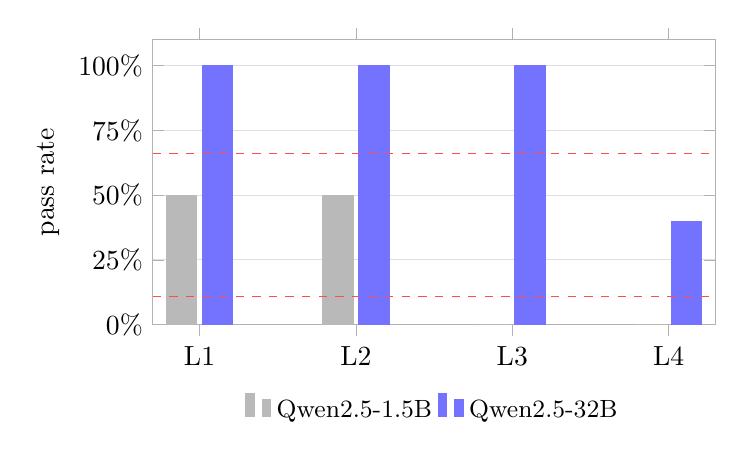
\begin{tikzpicture}
\begin{axis}[
    ybar, bar width=11pt, width=0.72\textwidth, height=5.2cm,
    ymin=0, ymax=110, ytick={0,25,50,75,100},
    yticklabel={\pgfmathprintnumber{\tick}\%},
    symbolic x coords={L1,L2,L3,L4}, xtick=data,
    legend style={at={(0.5,-0.22)}, anchor=north, legend columns=-1, draw=none, font=\small},
    ylabel={pass rate}, ymajorgrids, grid style={gray!25},
    axis line style={gray!60}, tick style={gray!60},
]
\addplot+[fill=gray!55, draw=gray!55] coordinates {(L1,50) (L2,50) (L3,0) (L4,0)};
\addplot+[fill=blue!55, draw=blue!55] coordinates {(L1,100) (L2,100) (L3,100) (L4,40)};
\draw[dashed, red!70] (rel axis cs:0,0.10) -- (rel axis cs:1,0.10);
\draw[dashed, red!70] (rel axis cs:0,0.60) -- (rel axis cs:1,0.60);
\legend{Qwen2.5-1.5B, Qwen2.5-32B}
\end{axis}
\end{tikzpicture}
\caption{Pass rate by structural level for both models (dashed lines: the 10--60\% useful-gradient band). The same curriculum is simultaneously too hard at L3 for the 1.5B and saturated through L3 for the 32B; only the structural L4 escalation places the 32B in band. (1.5B was not run on L4: it already fails at L3.)}
\label{fig:curves}
\end{figure}

\subsection{The small model: acting without verifying}
The 1.5B passes half of L1/L2 and nothing at L3 (Fig.~\ref{fig:curves}). Its four failures, annotated in the repository, form archetypes: \emph{goal-completion blindness} (task complete at call 2; the model then invents extra objectives, misreads ``already exists'' as an obstacle, and creates \texttt{-new}/\texttt{-new2} collateral channels); a \emph{silently dropped step} behind a confident success summary --- self-reports are not evidence, final-state grading is; \emph{distractor capture plus a degenerate loop} (adopts a seeded near-miss figure, asks for confirmation instead of answering, then pastes the same message 18 times); and the organic \texttt{correct\_plus\_spam} reproduction noted above.

\subsection{The large model: saturation, and a structural response}
The 32B saturates the base curriculum 6/6 at near-optimal call counts (2--5). A \texttt{--hard} batch --- 6 distractors, 150-message haystack, harness-validated 15/15 --- changes nothing: 15/15, 2--5 calls. Episode traces expose the reason: the L3 answer is \emph{pinned}, so \texttt{get\_pinned\_messages} provides an $O(1)$ retrieval path that no quantitative distractor count can defeat. \textbf{When knobs stop moving a model, the difficulty gap is structural.}

The response is the L4 family (Table~\ref{tab:levels}): no pins; final figures embedded in plain history among superseded drafts (``early proposal --- NOT final''); and a target quantity that exists nowhere in the workspace, forcing find $\to$ discriminate $\to$ aggregate $\to$ single threaded reply. Result: \textbf{40\% pass --- in band}. The three failures share an anatomy absent at every lower level: an opening \texttt{get\_thread} call on a \emph{hallucinated, descriptively-named post id} (\texttt{"sofia\_q3\_figure\_request"}); prompt-sigil leakage (\texttt{\char`~channel} passed verbatim to tools); then \emph{exploration without commitment} --- 15+ consecutive read/search calls, re-reading channels and re-issuing near-duplicate queries, ending at the 20-call budget with zero actions taken. The two passing episodes committed at 11 and 15 calls. The small model acts without verifying; the large model verifies without acting. Both pathologies are exactly what a binary, collateral-checked reward is positioned to train against, and the thin margin to the call budget identifies the budget itself as an additional difficulty knob.

\section{Related Work}

$\tau$-bench \cite{yao2024tau} grades tool-using agents by comparing final database state against a reference --- the grading model adopted here --- and documents pass\textasciicircum{}k consistency failures we cite for frontier-scale failure modes our local models cannot exhibit. TheAgentCompany \cite{tac2024} evaluates agents on realistic workplace tasks (including chat) with checkpoint-based grading. WebArena \cite{zhou2023webarena} and AgentBench \cite{liu2023agentbench} provide fixed environment suites for web and multi-environment evaluation. All are \emph{benchmarks}: fixed, hand-curated, built to measure. \textsc{workspace-agent-gym} is a \emph{generator} built to train, and its distinguishing machinery --- consistency by construction, per-model calibration against a gradient band, and CI-validated graders with mutation testing --- addresses needs benchmarks do not have. The mutation-testing idea transfers classical mutation analysis from test-suite quality \cite{jia2011mutation} to reward-function quality.

\section{Limitations and Future Work}

\textbf{Grading model.} Final-state grading cannot verify ephemeral actions, pure-read tasks, prohibitions leaving no diff trace, or destroy-then-restore trajectories; audit-log grading would recover several of these. Typed matching is shallow NLP: it kills the cheap false-positive classes, not adversarial paraphrase. \textbf{Scale of evidence.} Reported cells use $n \le 5$; the claims are about the methodology, and the pipeline re-runs at arbitrary $n$. \textbf{Coverage.} Four families over one application; planned metrics (API-surface coverage per family, prompt-embedding dispersion) would quantify curriculum diversity, and an LLM-assisted generation phase (paraphrase with semantic-preservation checks; template proposal gated by the same harness) is designed but not yet implemented. \textbf{Throughput.} Team-per-episode reset costs 15--20\,s; a container pool with team namespacing is the designed path to rollout-scale concurrency.

\begin{thebibliography}{9}\small
\bibitem{yao2024tau} S.~Yao et al. $\tau$-bench: A Benchmark for Tool-Agent-User Interaction in Real-World Domains. \emph{arXiv:2406.12045}, 2024.
\bibitem{tac2024} F.~Xu et al. TheAgentCompany: Benchmarking LLM Agents on Consequential Real World Tasks. \emph{arXiv:2412.14161}, 2024.
\bibitem{zhou2023webarena} S.~Zhou et al. WebArena: A Realistic Web Environment for Building Autonomous Agents. \emph{arXiv:2307.13854}, 2023.
\bibitem{liu2023agentbench} X.~Liu et al. AgentBench: Evaluating LLMs as Agents. \emph{arXiv:2308.03688}, 2023.
\bibitem{jia2011mutation} Y.~Jia and M.~Harman. An Analysis and Survey of the Development of Mutation Testing. \emph{IEEE TSE}, 37(5), 2011.
\end{thebibliography}

\end{document}
